%%%%%%%%%%%%%%%%%%%%%%% preamble %%%%%%%%%%%%%%%%%%%%%%%%%%%
\documentclass[10pt,letterpaper]{article}
\usepackage{opex3}
\usepackage{hyperref}
\usepackage{amssymb}
\hypersetup{colorlinks=true,
		      urlcolor=blue}
\usepackage{amsmath}      
\usepackage{bm}
\usepackage{listings}
\lstdefinestyle{mybashstyle}{
  language=Python,
  numbers=none,
  stepnumber=1,
  numbersep=10pt,
  tabsize=4,
  showspaces=false,
  showstringspaces=false,
  commentstyle=\color{light-gray},
  keywordstyle=\color{magenta},  
}
\lstset{
		emph={from, hadoop, fs, ls, put, get, mkdir, 
			text, copyFromLocal, copyToLocal,
			cp, mv, cat, appendToFile, select, and,
			where, set, true, false, done, do, hive,
			transform, using, limit, use, add
			},
%	morekeywords={hadoop, fs, ls, put, get, cat, copyToLocal, copyFromLocal},
	basicstyle={\ttfamily}, 
 	style=mybashstyle,
	emphstyle={\color{magenta}}
 }
\newcommand{\myeqno}[1]{Eq.~\eqref{#1}}
\DeclareMathOperator*{\argmin}{arg\,min}

%%%%%%%%%%%%%%%%%%%%%%% begin %%%%%%%%%%%%%%%%%%%%%%%%%%%%%%
%\linespread{1.25}
\begin{document}
\title{\Large{Assignment 2: Randomized optimization}}
\author{\href{mailto:rohan.kekatpure@gmail.com}{Rohan D. Kekatpure}}
\address{}
\email{}

\section{Organization of the report}
The present report comprises of two parts corresponding to homework description: (1) neural network training using randomized optimization techniques and (2) comparison of randomized optimized techniques using three discrete optimization problems. 

Since our origin neural network is implemented in R, we've used R for the first part. Specifically, the R libraries {\tt GenSA} and {\tt GA} are used for simulated annealing (SA) and genetic algorithm (GA) optimization respectively.

Unfortunately, these libraries have limited documentation for {\em discrete} optimization problems. So We've used the {\sc abagail} library for PART 2.   

\section{Part 1: Neural network weights}
Our neural network problem of choice is the Ionosphere problem in Assignment 1. This dataset contains 350 observations; each observation having 34 attributes. The objective is to classify each observation into a `good' and `bad' class. I believe the following factors qualify these datasets as `interesting':
\begin{enumerate}
	\item Ionosphere is a binary classification problem with 34 attributes. Its binary nature allows an easier comparative analysis of various binary classification algorithms.  
	\item Ionosphere data is small enough to allow us to efficiently train our models. 

For our studies, we include 150 observations in our training set and use the remaining 200 observations for testing. We don't know the train/test split use by the published studies, which might affect how closely we're able to reproduce these results.

\end{enumerate}

\subsection{Randomized hill climbing (RHC)}
Not implemented
%%
\subsection{Simulated annealing}
\subsubsection{Methodology}\label{meth1}
As mentioned above, the {\tt GenSA} package in R was used to implement the SA algorithm. The neural network itself was implemented using the {\tt nnet} package. Our network had 1 hidden layer and 10 hidden units. The {\tt GenSA} package provides the {\tt GenSA()} function which takes a vector of inputs as the first value and a callable ({\tt evalfunction}) as the second argument. Our {\tt evalfunction} was the squared error objective function value of the neural network. To implement {\tt evalfunction} we asked the {\tt nnet} package to simply evaluate the objective function without any training iterations. 
%%
\subsubsection{Results}
Figure~\ref{sal} shows the minimization of the objective function performed via the SA algorithm. The cost function value, after about 66,000 function evaluations has saturated at about $f_{\text{min}} = 71.1$. The optimization run took about 235 seconds and final training and the test error were about $1.49\%$ and $7.94\%$ (average of 10 runs). 

\begin{figure}[!htbp]
	\centering
	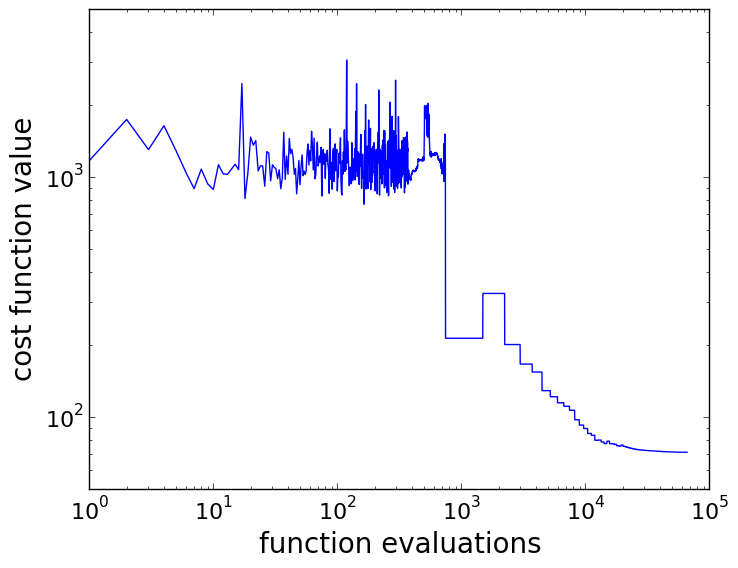
\includegraphics[width=3in]{../plots/simulatedannealing.png}
	\caption{Convergence of simulated annealing optimization. Initial temperature was 200. \label{sal}}
\end{figure}
\subsection{Genetic optimization}
\subsubsection{Methodology}
The general methodology was similar to \S\ref{meth1}. For the GA algorithm, we used the {\tt GA} package in R. The only difference here was that since the {\tt GA} package performs maximization, the cost function needed to be negated. 
%%
\subsubsection{Results}
Figure~\ref{gal} shows the best results for neural network cost function minimization performed via the GA algorithm with local arithmetic (LA) crossover. After about 240,000 function evaluations, the final function value of $C_{\text{min}}=88.53$ was obtained. This corresponded to a final training and test errors of $1.99\%$ and $16.56\%$ respectively. The wall clock time for the optimization problem was 1200 seconds. 

Compared to simulated annealing, we found it was more difficult to optimize the weights using GA. The performance above was the best we could obtain and it was after experimenting with four different crossover functions (described below) and a range of mutation probabilities. 

The {\tt GA} package in R provides a choice of four cross-over functions for real-value encoded GA problems. Below are the results of our experiments with each of the cross-ver methods. First we provide the results and analyze them together with simulated annealing in the next section.
%
\begin{enumerate}
\item Single-point crossover:
 This is the standard single-point method where two children ($c_1$ and $c_2$), each getting a contiguous part of the bit value of weights of two parents ($p_1$ and $p_2$). 
\begin{align}
c_1 &= p_1[1 : k] + p_2[k+1 : n] \nonumber \\
c_2 &= p_2[1 : k] + p_1[k+1 : n] \nonumber
\end{align}
where the operator `$+$' is overloaded to mean string concatenation.

Weights generated using a single-point crossover were suboptimal. The minimum cost function value obtained after varying the mutation probability from 10\% to 99\% was $f_{\text{min}}\sim 506$. Compare that with $f_{\text{min}}\sim 70$ obtained using backprop and simulated annealing. One possible reason for the bad performance of single-point crossover GA is that perhaps this crossover method is not well suited for real-valued features. After all what is the interpretation of generating floating points by crossing over bit patterns? In fact, for small weights ($\simeq 1.0$), a half-way single-point cross often (but not always) produces children that are identical to parents. This fact can be verified by the Python script in the Appendix. This greatly undermines the crossover operation. Despite these limitations, the {\tt GA} package provides it as an option for real-valued features. 
%%
\item Local arithmetic (LA) crossover:
 This crossover method generates two children from two parents by altering only a few features (co-ordinates) of the parents. The alternation consists of performing a linear combination of parent features. For example if the two parents are:
\begin{align}
    p_1 &= (x_1, x_2, \ldots, x_n) \nonumber \\
    p_2 &= (y_1, y_2, \ldots, y_n) \nonumber
\end{align}
then the children are
\begin{align}
    c_1 &= (x_1, x_2, \ldots,\alpha x_k + (1-\alpha)y_k, \ldots, x_n) \nonumber \\
    c_2 &= (y_1, y_2, \ldots,\alpha y_k + (1-\alpha)x_k, \ldots, y_n) \nonumber 
\end{align}

For the LA crossover, I went with the default settings and varied mutation probability between 10\% and 99\%. We obtained best performance with LA crossover with {\tt pmutation} = 99\%. Figure~\ref{gal} represents the 240,000 iteration of the genetic algorithm with LA crossover.   
%%
\item Whole arithmetic (WA) crossover: 
 The WA crossover is similar to LA crossover except the entire parent vector is used.
\begin{align}
    p_1 &= (x_1, x_2, \ldots, x_n) \nonumber \\
    p_2 &= (y_1, y_2, \ldots, y_n) \nonumber \\
    c_1 &= \alpha p_1 + (1-\alpha)p_2 \nonumber \\
    c_2 &= (1-\alpha) p_1 + \alpha p_2
\end{align} 
WA crossover worked significantly better than single-point crossover, but 50\% as worse compared to LA crossover. The cost function minimum obtained using WA crossover at {\tt pmutation}=99\% is $f_{\text{min}}=150$. It appears that big deviations from parents don't lead to a better search performance. 
%%
\item Blended crossover (BLX):
 Blended crossover expands the search boundary and adds a mutation-like randomness. Assume the parents, like before, are $n$-component real-valued feature vectors. 
\begin{align}
    p_1 &= (x_1, x_2, \ldots, x_n) \nonumber \\
    p_2 &= (y_1, y_2, \ldots, y_n) \nonumber
\end{align}  
Define 
\begin{align*}
d_i &= \vert x_i -y_i \vert  \\
m_i &= \min(x_i, y_i) -\alpha d_i \\
M_i &= \max(x_i, y_i) +\alpha d_i 
\end{align*}
Components $x_i$ and $y_i$ for the next generation are chosen uniformly randomly from the interval $[m_i,\, M_i]$. 

BLX crossover performed slightly better than single-point crossover but significantly worse then WA and (therefore) LA crossovers. Cost function minimum obtained using BLX crossover at {\tt pmutation} = 99\% is $f_{\text{min}}=350$.
\end{enumerate} 
%%
\begin{figure}[htbp]
	\centering
	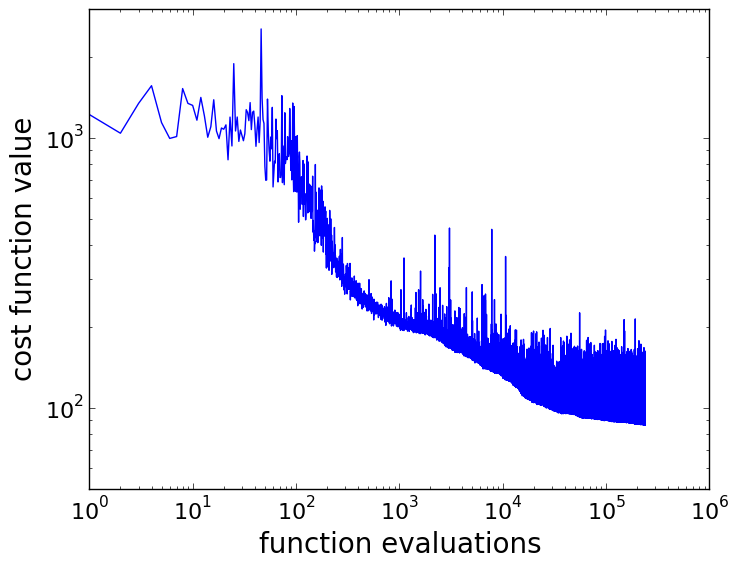
\includegraphics[width=3in]{../plots/geneticalgorithm.png}
	\caption{Convergence of genetic algorithm with LA crossover and {\tt pmutation} = 99\%. \label{gal}}
\end{figure}
%%
\subsection{Summary and discussion}
\begin{table}[htbp]
	\caption{ Comparison of simulated annealing and genetic algorithms with different crossover functions. \label{tab1}}
	\centering
    \begin{tabular}{p{3cm}|p{1.5cm}|p{1cm}|p{2.2cm}|p{2.cm}}
         \hline
            	{\bf Algorithm} & {\bf Training time} & {$f_{\text{min}}$} & {\bf Training error} & {\bf Test error}\\ \hline \hline
	         Backpropogation & 10 s & 70.5 & 1.49\% & 6.5\% \\ \hline
		Simulated annealing & 235 s & 72.8 & 1.49\% & 7.9\%\\ \hline
		GA, SP crossover & 1200 s & 450& 23.4\% & 45.2\%\\ \hline
		GA, LA crossover & 1200 s & 88.5 & 1.99\% & 16.5\%\\ \hline
		GA, WA crossover & 1200 s & 168.3 & 13.4\% & 32.4\%\\ \hline
		GA, BLX crossover & 1200 s & 345.2 & 20.1\% & 39.5\%\\ \hline
    \end{tabular}
\end{table}
In general, randomized optimization approaches take significantly longer computation times compared with direct approaches like backpropagation. The obtained solutions are also suboptimal. However, memory or computational constraints might mandate the use of randomized optimization algorithms.

Simulated annealing (SA) algorithm achieved almost the same $f_{\text{min}}$ and test error as Backpropagation, but took almost a hundred times longer to compute because of random search. One technique to reduce the run time is to apply a faster cooling rate. Unfortunately the {\tt GenSA} package does not seem to allow altering the cooling rate. The documentation \footnote{https://cran.r-project.org/web/packages/GenSA/GenSA.pdf} has no mention of this control parameter. One of the publication by the {\tt GenSA} team \footnote{https://journal.r-project.org/archive/2013-1/xiang-gubian-suomela-etal.pdf} mentions that the cooling rate can be altered by passing the argument, but there is no example in the documentation or the general web showing how to do that. As a result I was unable to experiment with this parameter. Another technique might be to cache function values to avoid repeated function computations. However, it is unclear how we can do that since we're dealing with a multidimensional real values feature vector at machine precision (e.g. evaluation is requested at $x = 1.5$ but value in lookup table is at $x = 1.45$. Lookup is even less beneficial in multiple dimensions.) 

Our SA experiments were therefore limited to varying the initial temperature. All of these yielded approximately similar performance indicating that there aren't any faraway maxima. 

Genetic algorithms performed worse by comparison both when evaluated by computation time as well as final results. We experimented with two parameters: (1) four different crossover functions and (2) varying mutation probability from 0.10 to 0.99. A mutation probability close to 1 was {\em necessary} to obtain a minimum function value; without that the results were much worse than reported in Table~\ref{tab1}. Local arithmetic (LA) crossover provided best performance.

Mutations in genetic algorithms allow for searching a small area around the current location by providing a small random wiggle room around the current location. Crossovers, on the other hand, provide an ability to make large leaps  somewhere `in between' the parents. Also, for real-valued inputs, mutation adds random new information to the solution, whereas crossovers combine already available information. 

Taking both the above observations into account, it seems that our neural network cost function has relatively sharp minimums, which can be captured only if our optimization algorithm has ability to perform random search around in its current vicinity. This reasoning can also be applied to understand the variation in the performance of different crossover functions. The single-point crossover does not result in different offspring for small floating-point inputs. The LA crossover makes very small alterations to the parent genes and therefore results in children that resemble the parents closely. WA and BLX crossovers, on the other hand, make large changes to parent genes and result in children far off from their parents, preventing  local search. 

\section{Part 2: Three discrete optimization problems}
\subsection{Algorithm evaluation method}
In part 2 of the assignment, we study three algorithms, each highlighting strengths of genetic algorithm (GA), simulated annealing (SA) and MIMIC. Different aspects can be stressed in evaluating the strength of an algorithm and defining a figure of merit for its measurement. One can consider the achieved final (maximized) value of the objective function, $f_{\text{max}}$. However, this ignores the cost in terms of time. After all, given infinite time, even a random hill climbing algorithm can find the global maximum. Therefore one also needs to consider the runtime of the algorithm. Runtime can be impacted by two independent factors. Either the function could be very expensive to evaluate or the function landscape could have a lot of local minima which necessitate a lot of iterations from some `naive' algorithms such as GA and SA. `Naive' here is used in the sense of throwing away information from function evaluations. 

If the total runtime is limited by expensive function evaluations, a general improvement strategy may be to use a method like MIMIC which extracts more information from function evaluations. If the total runtime is limited by cost function landscape then it might be more effective (time wise) to use relatively faster methods like SA or GA. 

To evaluate the various algorithms, we'll plot $f_{\text{max}}$ vs runtime. The number of iterations is the implicit parameter in all these plots since each value of runtime and $f_{\text{max}}$ is obtained by varying the number of iterations. In this scheme, the best algorithm is that which obtained largest $f_{\text{max}}$ in least amount of runtime. So on a graph of $f_{\text{max}}$ on the $y$ axis and runtime on the $x$ axis, the best algorithm would be on the top left (max value in min time).

The first two problems (count ones and Rastrigin function) demonstrate strength of the Simulated annealing method, the next two (traveling salesman and four peaks) demonstrate the strengths of MIMIC and the last problem highlights the strength of genetic algorithm.

\subsection{Count ones}
The count ones is an already implemented algorithm in the {\sc abagail} package. The input to this function is bit strings and the objective function value is simply the number of 1's in the string. This function is easy to evaluate, but not necessarily easy to optimize. For our test we used 100 bit strings so $f_{\text{max}} = 100$. Figure~\ref{part2}(a) shows the results of running the three algorithms on the CountOnes problem. It is clear that simulated annealing outperforms the other algorithms for this problem. The reasons are exactly as mentioned previously: CountOnes objective function is easily evaluated and trading off number of function evaluations for costlier sampling in MIMIC is not warranted. 
\subsection{Rastrigin test}
Rastrigin test problem can be thought of as a continuous as well as a discrete optimization problem. Here we evaluate is as a real-valued cost function of discrete inputs. It is defined as: 
\begin{align*}
x &= (x_1, x_2, \ldots, x_n)\\
R(x) &= nA + \sum_{i=1}^{n}\left[x_i^2 - A\cos(2\pi x_i)\right]\\
f(x) &= B -R(x)
\end{align*}
$R(x)$ is the actual Rastrigin function (As defined in the \href{https://en.wikipedia.org/wiki/Rastrigin_function}{Wikipedia}). We've modified it by adding the last equation for $f(x)$ which merely converts a minimization problem into a maximization. Our modified Rastrigin function, as defined above, has a global maximum at $x = (0,0, \ldots, 0)$ with the value  $f_{\text{max}} = B$.

For our experiments, we used $n=100$ and $A=10$. Rastrigin function has a relatively shallow global maximum and is surrounded on all sides by local maximums. As such, it is a difficult optimization problem. However, the function evaluation itself is not particularly costly. Because of this characteristic, simulated annealing once again outperforms MIMIC as seen in Figure~\ref{part2}(b). Note that both MIMIC and SA solve the problem (i.e. achieve $f_{\text{max}}=100$, but SA achieves it 100 times faster. Notably, in our experiments, genetic algorithm is unable to solve the problem with either a single-point crossover or a uniform crossover. Upon monitoring the GA solution, we found that the algorithm gets stuck in one of the local maxima, whose location is dependent on the choice of initial position.

Our next two optimization problems illustrate the strengths of MIMIC.
\subsection{Traveling salesman}
Travaling salesman cost function is costly to evaluate. As such, it is chosen so that SA and GA techniques, which require relatively more function evaluations, would not be able to solve it in our number of allowed iterations. This is exactly what we observed in our experiments. As seen in Figure~\ref{part2}(c), MIMIC clearly outperforms SA and GA in finding the maximum value. Both the latter algorithms are unable to find the optimum solution in the maximum allotted 5000 iterations. SA and GA find similar (sub)optimum values  but SA reaches there faster.
%%
\subsection{Four peaks}
We used a four peaks (FP) problem with an array of dimension $N=200$ and $T = 20\%$. The \href{http://www.cc.gatech.edu/~isbell/tutorials/mimic-tutorial.pdf}{four peaks problem} illustrates strengths of MIMIC in a different way. While the FP function itself is not particularly costly to evaluate, it has two broad basins of attraction which tend to trap SA and GA in local maxima. The regions of sample space that MIMIC eliminates in every iteration prove crucial to its ability to reach the {\em global} maximum. As Figure~\ref{part2} shows, in our allotted 5000 iterations, none of the algorithm has achieved $f_{\text{max}}$, but MIMIC is close to achieving the theoretical maximum of $f_{\text{max}} = 240$. 
%%
\subsection{Knapsack problem}
The knapsack problem we chose has 40 items with 4 copies each and the maximum weight is restricted to 50. For the knapsack problem, all three algorithms perform almost equally. However, GA performs {\em slightly} better, as seen from Figure~\ref{part2}(e). However, this advantage seems marginal when compared to its increased time in comparison to SA.

This is a general observation about SA and GA. We were hard-pressed to come up with problem in which GA outperformed SA in terms of runtime and convergence rate. Research articles comparing the two algorithms also conclude similarly (\href{http://www.cs.helsinki.fi/u/kohonen/papers/gasa.html}{paper}).

One reason for a lack of clear benefit for GA may be that there is no obvious reason why GA's mutation + crossover strategy for `escaping' local optimums is better than SA. Also the choice of mutations and crossover functions provide more knobs to GA, which must be precisely tuned (much like hyperparameters). Any suboptimal choice of mutation and crossover functions can severely impact performance of GA. In spite of this, there is no systematic procedure for scanning though different mutation and crossover functions. 

In our present studies, we retained the default mutation strategy, but experimented with uniform and single-point crossover. However, the choice of crossover function did not provide any visible benefit to the problem solution.

\subsection{General observations}
From Figure~\ref{part2} it seems that if a problem is solvable for SA, it will be the fastest one to solve it. However, throwing more runtime at SA (i.e. increasing the number of iterations) does not necessarily lead to an improved performance for SA. In that sense it is stochastic. This is because SA is sampling the entire space for every iterations, including the regions where the function value is not likely to be optimum. 

MIMIC, on the other hand, approaches the optimum value much more systematically. This is built into the algorithm. It successively eliminates the `suboptimal' regions of the search space and retains only the regions where the optimum will be found. As a result, with MIMIC, we can be confident that any extra runtime thrown at the algorithm is likely to be beneficial. This is an important confidence to have in an algorithm.
\begin{figure}[!h]
	\begin{center}
	 \makebox[\textwidth][c]{%
		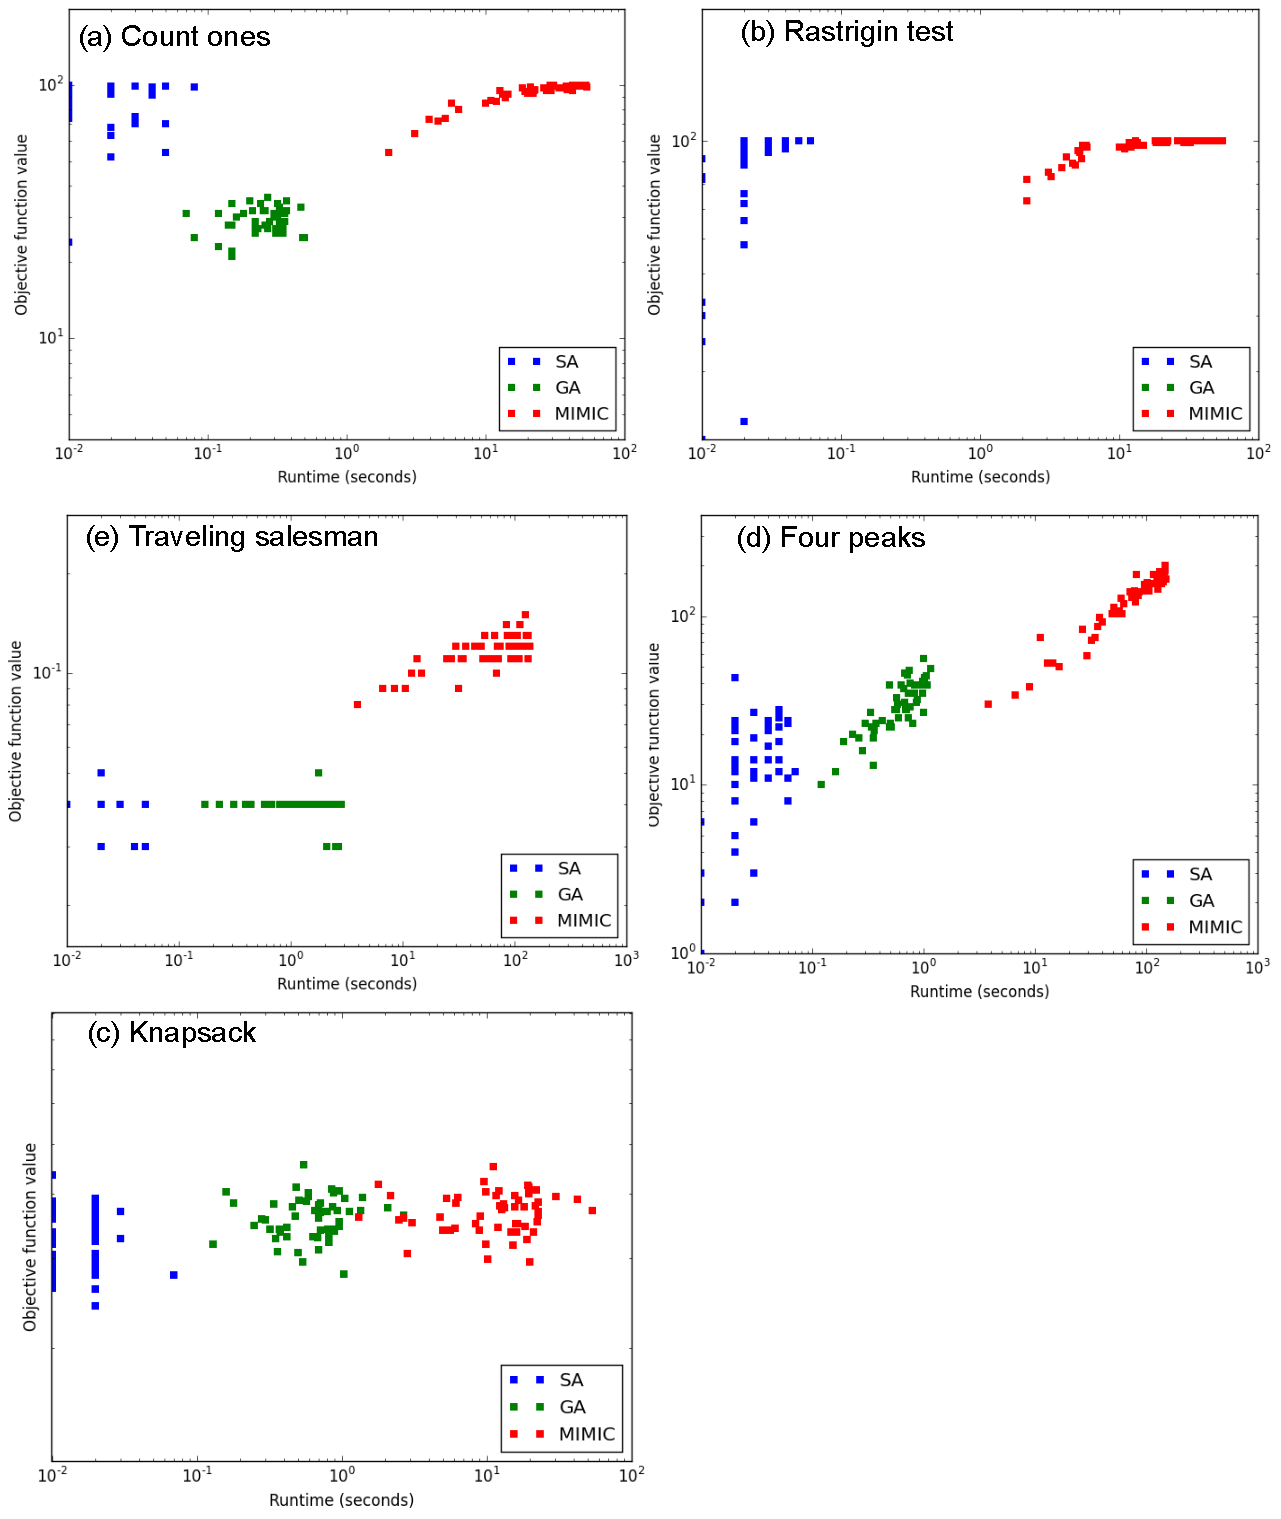
\includegraphics[width=7in]{../plots/part2.pdf}
          }
	\caption{Maximization of various discrete functions described in the text: (a) count ones (b) Four peaks (c) Knapsack (d) Rastrigin and (e) Traveling salesman. The blue, green and red plots correspond to results of simulated annealing, genetic algorithm and MIMIC respectively. The results of genetic algorithm are not visible in part (d) because of the scale used. \label{part2}}
	\end{center}
\end{figure}

\section*{Appendix: Python script to perform single-point crossover}
\begin{scriptsize}
\begin{lstlisting}[language=python]
import struct
def float_to_bits(fnum):
    hexnum = struct.pack('>f', fnum)
    bits = ''.join([bin(ord(c))
    	     .replace('0b', '')
    	     .rjust(8, '0') 
    	     for c in hexnum])
    return bits

def spxover(f1, f2, k):
    f1_bits = float_to_bits(f1)
    f2_bits = float_to_bits(f2)
    c1_bits = f1_bits[:k] + f2_bits[k:]
    c2_bits = f2_bits[:k] + f1_bits[k:]
    return f1_bits, f2_bits, c1_bits, c2_bits

if __name__ == '__main__':
	f1 = 1.0
	f2 = 2.0
	f1b, f2b, c1b, c2b = spxover(f1, f2, 16)
	if f1b == c1b:
		print "f1b == c1b"

	if f2b == c2b:
		print "f2b == c2b"
\end{lstlisting}
\end{scriptsize}
\end{document}













